\documentclass[epsfig,10pt,fullpage]{article}

\newcommand{\LabNum}{7}
\newcommand{\CommonDocsPath}{../../../../common/docs}
\addtolength{\textwidth}{1.5in}
\addtolength{\oddsidemargin}{-0.75in}
\addtolength{\topmargin}{-0.75in}
\addtolength{\textheight}{1.5in}
\addtolength{\evensidemargin}{0.75in}
\setlength\parindent{0pt}
\raggedbottom

\usepackage{ae,aecompl}
\usepackage{epsfig,float,times}
\usepackage[hypcap]{caption}
\usepackage[pdftex, colorlinks]{hyperref}
\usepackage{graphicx}
\usepackage[usenames, dvipsnames]{color}
\usepackage{rotating}
\usepackage{tikz}
\usetikzlibrary{automata,positioning}
\usepackage{placeins}

\widowpenalty 10000
\clubpenalty 10000

\newcommand{\red}[1]{{\color{red}\sf{#1}}}
\newcommand{\green}[1]{{\color{green}\sf{#1}}}
\newcommand{\blue}[1]{{\color{blue}\sf{#1}}}
\definecolor{PineGreen}{rgb}{0.0, 0.47, 0.44}
\definecolor{ForestGreen}{rgb}{0.13, 0.55, 0.13}
\definecolor{Brown}{rgb}{0.59, 0.29, 0.0}

\newcommand{\UPDatePublished}{Oct 2021}
\newcommand{\versnum}{21.1} %version number quartus/AMP
\newcommand{\quartusname}{Quartus\textsuperscript{\textregistered} Prime}	
\newcommand{\UPTextBar}{For \quartusname{} \versnum{}}
\newcommand{\thisyear}{2021 } %for copyright
\newcommand{\company}{FPGAcademy.org}
\newcommand{\longteamname}{FPGAcademy.org}
\newcommand{\teamname}{FPGAcademy}
\newcommand{\website}{FPGAcademy.org}

\newcommand{\productAcronym}{AMP}
\newcommand{\productNameShort}{Monitor Program}

\newcommand{\productNameMedTM}{A Monitor Program}
\newcommand{\productNameMed}{A Monitor Program}

%\newcommand{\headerLogoFilePath}[1]{#1/FPGAcademy.png}

% listings is a package that supports encapsulating source code in LaTeX conveniently
\usepackage{listings}

\def\expandparam\lstinputlisting[#1]#2{\edef\tmp{\noexpand\lstinputlisting[#1]{#2}}\tmp}

%%%%%%%%%%%%%%%%%%%% Source Code Formatting %%%%%%%%%%%%%%%%%%%%
\definecolor{globalCommentColour}{rgb}{0.588,0.588,0.588}

%%%%%%%%%%%%%%%%%%%%%%%%%%%%%%%%%%%%%%%%%%%%%%%%%%%%
% Defining language style
% NiosII ASM
\lstdefinelanguage[NiosII]{Assembler} {
  morekeywords={add, addi, and, andhi, andi, beq, bge, bgeu, bgt, bgtu, ble,  bleu, blt, bltu, bne, br, break,
  bret, call, callr, cmpeq, cmpeqi, cmpge, cmpgei, cmpgeu, cmpgeui, cmpgt, cmpgti, cmpgtu, cmpgtui, cmple,
  cmplei, cmpleu, cmpleui, cmplt, cmplti, cmpltu, cmpltui, cmpne, cmpnei, custom, div, divu, eret, flushd,
  flushda, flushi, flushp, initd, initda, initi, jmp, jmpi, ldb, ldbio, ldbu, ldbuio, ldh, ldhio, ldhu, ldhuio,
  ldw, ldwio, mov, movhi, movi, movia, movui, mul, muli, mulxss, mulxsu, mulxuu, nextpc, nop, nor, or, orhi, ori,
  rdctl, rdprs, ret, rol, roli, ror, sll, slli, sra, srai, srl, srli, stb, stbio, sth, sthio, stw, stwio,
  sub, subi, sync, trap, wrctl, wrtcl, wrprs, xor, xori, xorhi, xori},
  morekeywords=[2]{.abort, .ABORT, .align, .app-file, .ascii, .asciz, .balign, .byte, .comm, .data, .def,
  .desc, .dim, .double, .eject, .else, .end, .endef, .endif, .equ, .equiv, .err, .extern, .file, .fill, .float,
  .global, .globl, .hword, .ident, .if, .include, .int, .irp, .irpc, .lcomm, .lflags, .line, .linkonce, .ln,
  .list, .long, .macro, .mri, .nolist, .octa, .org, .p2align, .psize, .quad, .rept, .sbttl, .scl, .section,
  .set, .short, .single, .size, .sleb128, .skip, .space, .stadb, .stabn, .stabs, .string, .symver, .tag,
  .text, .title, .type, .val, .uleb128, .word},
  morekeywords=[3]{et, bt, gp, sp, fp, ea, sstatus, ra, pc, status, estatus, bstatus, ienable, ipending, cpuid,
  exception, pteaddr, tlbacc, tlbmisc, eccinj, badaddr, config, mpubase, mpuacc},
  sensitive=t,
  alsoletter=.,
  morestring=[b]",
  morecomment=[s]{/*}{*/},
  morecomment=[l]\#,
}[keywords,comments,strings]
   
%% NOTE: morekeywords=[2] are GNU directives.
   
\definecolor{niosInstructionColour}{rgb}{0.000,0.608,0.000}
\definecolor{niosDirectiveColour}{rgb}{0.000,0.000,0.902}
\definecolor{niosSpecialRegColour}{rgb}{0.000,0.000,0.000}
\definecolor{niosStringColour}{rgb}{0.808,0.482,0.000}
   
%% NOTE: To make bold use: =\bfseries\color{<colour>}
\lstdefinestyle{defaultNiosStyle} {
  language=[NiosII]{Assembler},
  stringstyle=\color{niosStringColour},
  keywordstyle=\color{niosInstructionColour},
  keywordstyle=[2]\color{niosDirectiveColour},
  keywordstyle=[3]\itshape\color{niosSpecialRegColour}
}
%%%%%%%%%%%%%%%%%%%%%%%%%%%%%%%%%%%%%%%%%%%%%%%%%%%%

%%%%%%%%%%%%%%%%%%%%%%%%%%%%%%%%%%%%%%%%%%%%%%%%%%%%
% Defining language style
% ArmA9 ASM
\lstdefinelanguage[ArmA9]{Assembler} {
  morekeywords={ADC, ADD, ADDS, AND, ANDS, B, BAL, BEQ, BGE, BGT, BL, BLT, BIC, BKPT, BLX, BNE, BX, CDP, CLZ, CMN, CMP, EOR,
  EORS, LDC, LDM, LDR, LDRB, LDRBT, LDRH, LDRSB, LDRSH, LDRT, LSL, MCR, MLA, MOV, MOVW, MOVT, MRC, MRS, MSR, MUL, MVN, ORR, PLD,
  ROR, RSB, RSC, SBC, SMLAL, SMULL, STC, STM, STR, STRB, STRBT, STRH, STRT, SUB, SUBS, SWI, SWP, SWPB, TEQ, UMLAL,
  PUSH, POP, MOVS, RORS, LSR},
  morekeywords=[2]{.abort, .ABORT, .align, .app-file, .ascii, .asciz, .balign, .byte, .comm, .data, .def,
  .desc, .dim, .double, .eject, .else, .end, .endef, .endif, .equ, .equiv, .err, .extern, .file, .fill, .float,
  .global, .globl, .hword, .ident, .if, .include, .int, .irp, .irpc, .lcomm, .lflags, .line, .linkonce, .ln,
  .list, .long, .macro, .mri, .nolist, .octa, .org, .p2align, .psize, .quad, .rept, .sbttl, .scl, .section,
  .set, .short, .single, .size, .sleb128, .skip, .space, .stadb, .stabn, .stabs, .string, .symver, .tag,
  .text, .title, .type, .val, .vectors, .uleb128, .word},
  morekeywords=[3]{SP, PC, MIDR, CTR, TCMTR, TLBTR, MPIDR, ID_PFR0, ID_PFR1, ID_DFR0, ID_MMFR0, ID_MMFR1, ID_MMFR2,
  ID_MMFR3, ID_ISAR0, ID_ISAR1, ID_ISAR2, ID_ISAR3, ID_ISAR4, CCSIDR, CLIDR, AIDR, CSSELR, TTBR0, TTRB1, TTBR2, DACR,
  DFSR, IFSR, ADFSR, AIFSR, DFAAR, IFAR, ICIALLUIS, BPIALLIS, PAR, ICIALLU, ICIMVAU, BPIALL, DCIMVAC, DCISW, V2PCWPR,
  DCCVAC, DCCSW, DDIMVAC, DCISW, TLBALLIS, TLBIMVAIS, TLBIASIDIS, TLBIMVAAIS, TLBIALL, TLBIMVA, TLBIASID, TLBIMVAA,
  PMCR, PMCNTENSET, PMCNTENCLR, PMOVSR, PMSWINC, PMSELR, PMXEVTYPER, PMXEVCNTR, PMUSERENR, PMINTENSET, PMINTENCLR,
  PRRR, NRRR, PLEIDR, PLEASR, PLEFSR, PLEUAR, PLEPCR, VBAR, MVBAR, ISR, FCSEIDR, CONTEXTIDR, TPIDRURW, TPIDRURO, TPIDRPRW},
  sensitive=f,
  alsoletter=.,
  morestring=[b]",
  morecomment=[s]{/*}{*/},
  morecomment=[l]{//},
}[keywords,comments,strings]
   
%% NOTE: morekeywords=[2] are GNU directives.
   
\definecolor{armInstructionColour}{rgb}{0.000,0.608,0.000}
\definecolor{armDirectiveColour}{rgb}{0.000,0.000,0.902}
\definecolor{armSpecialRegColour}{rgb}{0.000,0.000,0.000}
\definecolor{armStringColour}{rgb}{0.808,0.482,0.000}
   
\lstdefinestyle{defaultArmStyle} {
  language=[ArmA9]{Assembler},
  stringstyle=\color{armStringColour},
  keywordstyle=\color{armInstructionColour},
  keywordstyle=[2]\color{armDirectiveColour},
  keywordstyle=[3]\itshape\color{armSpecialRegColour}
}
%%%%%%%%%%%%%%%%%%%%%%%%%%%%%%%%%%%%%%%%%%%%%%%%%%%%

%%%%%%%%%%%%%%%%%%%%%%%%%%%%%%%%%%%%%%%%%%%%%%%%%%%%
% Defining language style
% FPGAcademy ASM
\lstdefinelanguage{ASM}{
  morekeywords = [1]{mv, mvt, mvne, mvcc, add, sub, st, ld, and, b, bne, beq, bcc, bcs},
  morekeywords = [2]{word, define},
  keywordstyle = [1]\color{ForestGreen},
  keywordstyle = [2]\color{blue},
  sensitive = true,
  morecomment = [l]{//},
}

\lstset{
  language = ASM,
  basicstyle=\small\color{black}\ttfamily,
  commentstyle=\small\color{Brown}\itshape\ttfamily,
  showstringspaces=false,
  frame=none, %lines % boxed listings
  breaklines=true,
  breakatwhitespace=true,
  tabsize=3
}
%%%%%%%%%%%%%%%%%%%%%%%%%%%%%%%%%%%%%%%%%%%%%%%%%%%%

%%%%%%%%%%%%%%%%%%%%%%%%%%%%%%%%%%%%%%%%%%%%%%%%%%%%
% Defining language style
% Java
\definecolor{javaStringColour}{rgb}{0.808,0.482,0}
%%%%%%%%%%%%%%%%%%%%%%%%%%%%%%%%%%%%%%%%%%%%%%%%%%%%

%%%%%%%%%%%%%%%%%%%%%%%%%%%%%%%%%%%%%%%%%%%%%%%%%%%%
% Defining language style
% C
\definecolor{CStringColour}{rgb}{0.808,0.482,0}

\lstset{
  language = C,
  basicstyle=\small\color{black}\ttfamily, 
  commentstyle=\small\color{PineGreen}\itshape\ttfamily,
  keywordstyle=\small\color{blue}\bfseries\ttfamily,
  showstringspaces=false,
  frame=none, %lines % boxed listings
  breaklines=true,
  breakatwhitespace=true,
  tabsize=3
}
%%%%%%%%%%%%%%%%%%%%%%%%%%%%%%%%%%%%%%%%%%%%%%%%%%%%

%%%%%%%%%%%%%%%%%%%%%%%%%%%%%%%%%%%%%%%%%%%%%%%%%%%%
% Defining language style
% Verilog
\definecolor{verilogCommentColour}{rgb}{0.000,0.502,0.000}

\lstdefinestyle{defaultVerilogStyle} {
  language={Verilog},
  keywordstyle=\color{blue},
  commentstyle=\color{verilogCommentColour}
}
%%%%%%%%%%%%%%%%%%%%%%%%%%%%%%%%%%%%%%%%%%%%%%%%%%%%

%%%%%%%%%%%%%%%%%%%%%%%%%%%%%%%%%%%%%%%%%%%%%%%%%%%%
% Defining language style
% VHDL
\lstdefinestyle{defaultVHDLStyle} {
  language={VHDL},
  keywordstyle=\color{blue},
  commentstyle=\color{verilogCommentColour}
}
%%%%%%%%%%%%%%%%%%%%%%%%%%%%%%%%%%%%%%%%%%%%%%%%%%%%

%%%%%%%%%%%%%%%%%%%%%%%%%%%%%%%%%%%%%%%%%%%%%%%%%%%%
% Defining language style
% LaTeX
\lstdefinelanguage[LocalLaTeX]{TeX}[LaTeX]{TeX}{moretexcs={bf, it, sf, lstset},}

\lstdefinestyle{defaultLocalLatexStyle} {
  language=[LocalLatex]{TeX},
  keywordstyle=\color{blue}\bfseries,
  keywordstyle=[2]\color{blue},
  keywordstyle=[3]\color{blue}\bfseries
}
%%%%%%%%%%%%%%%%%%%%%%%%%%%%%%%%%%%%%%%%%%%%%%%%%%%%

%%%%%%%%%%%%%%%%%%%%%%%%%%%%%%%%%%%%%%%%%%%%%%%%%%%%
% Defining language style
% Default
\lstset{
  basicstyle=\small\color{black}\ttfamily,
  commentstyle=\small\color{globalCommentColour}\itshape\ttfamily,
  keywordstyle=\small\color{blue}\bfseries\ttfamily,
  showstringspaces=false,
  frame=none, %lines % boxed listings
  breaklines=true,
  breakatwhitespace=true,
  tabsize=3
}
%%%%%%%%%%%%%%%%%%%%%%%%%%%%%%%%%%%%%%%%%%%%%%%%%%%%


\hypersetup{
  pdftitle={Computer Organization Lab Exercise \LabNum},
  linkcolor=blue,
  hyperindex=true,
  pdfauthor={FPGAcademy.org},
  pdfkeywords={FPGAcademy.org, FPGAcademy, Lab, Exercise, Computer Organization},
  bookmarks,
  bookmarksopen=false,
  filecolor=blue,
  pdfstartview={FitH},
  urlcolor=blue,
  plainpages=false,
  pdfpagelabels=true,
  linkbordercolor={1 1 1} %no color for link border
}



\begin{document}

\centerline{\huge Computer Organization}
~\\
\centerline{\huge Laboratory Exercise \LabNum}
~\\
\centerline{\large Using Interrupts with C code}
~\\

\noindent
The purpose of this exercise is to investigate the use of interrupts for the ARM* A9
processor, using C code. To do this exercise you need to be familiar with
the exceptions processing mechanisms of the ARM processor, and with the operation of
the ARM Generic Interrupt Controller (GIC). These concepts are discussed in the tutorials 
{\it Introduction to the ARM Processor}, and {\it Using the ARM Generic Interrupt
Controller}. We assume that you are using either the DE1-SoC, or DE10-Standard Computer
to implement the solutions to this exercise. It may be useful to read the parts of the 
documentation for those computer systems that pertain to the use of exceptions and interrupts.

~\\
\noindent
This exercise involves the same tasks as those given in Exercise 5,
except that this exercise uses C code rather than assembly-language code.
~\\
~\\
\noindent
{\bf Part I}
~\\
~\\
\noindent
Consider the main program shown in Figure~\ref{fig:code}. The program first initializes the
ARM A9 stack pointer for IRQ (interrupt) mode by calling a subroutine named
{\it set\_A9\_IRQ\_stack()}. This step is necessary because, although
the C compiler automatically generates code that initializes the SVC-mode (supervisor mode)
stack pointer, the C compiler does not generate code to initialize the IRQ-mode stack pointer.
The main program then calls subroutines {\it config\_GIC()} to initialize the generic 
interrupt controller (GIC), and {\it config\_KEYs()} to initialize the pushbutton KEYs 
port so that it will generate interrupts. 
Finally, a subroutine {\it enable\_A9\_interrupts()} is called to unmask
IRQ interrupts in the ARM processor. You are to fill in the missing code for the 
subroutines in Figure~\ref{fig:code}. After completing the initialization steps
described above, the main program just ``idles'' in an endless loop.

~\\
\noindent
The purpose of your program is to show the numbers \red{0} to \red{3} on the {\it HEX}0
to {\it HEX}3 displays, respectively, when a corresponding pushbutton {\it KEY} is pressed. 
Since the main program only idles in a loop, you have to control the displays by using an 
interrupt service routine for the pushbutton KEYs port.  Perform the following:

\begin{enumerate}
\item Create a new folder to hold your solution for this part. Create a
file, such as {\it part1.c}, for your main program, and create any other source-code files 
that you may wish to use.  Write the code for the subroutines that are called by the 
main program. For the {\it config\_GIC()} subroutine set up the
GIC to send interrupts to the ARM processor from the pushbutton KEYs port. 

\item 
Figure~\ref{fig:irq_code} gives the C code required for the interrupt handler. 
It is declared with the {\bf \_$\,$\_attribute\_$\,$\_} specification {\it interrupt}, 
and has the special name 
{\it \_$\,$\_cs3\_isr\_irq}.  Using this declaration allows the C compiler to recognize the 
code as being the IRQ interrupt handler. The compiler generates an entry corresponding
to this code in the ARM exception-vector table. 
  
You have to write the code for the {\it pushbutton\_isr()} interrupt service routine.
Your code should show the digit \red{0} on the {\it HEX}0 display when {\it KEY}$_0$ is
pressed, and then if {\it KEY}$_0$ is pressed again the display should be ``blank''. You should
toggle the {\it HEX}0 display between \red{0} and ``blank'' in this manner each time 
{\it KEY}$_0$ is pressed. Similarly, toggle between ``blank'' and \red{1}, \red{2}, or 
\red{3} on the {\it HEX}1 to {\it HEX}3 displays each time {\it KEY}$_1$, {\it KEY}$_2$,
or {\it KEY}$_3$ is pressed, respectively. 

The bottom part of Figure~\ref{fig:irq_code} provides code, using simple loops, which can 
be used for the other ARM exception handlers. Including these handlers in your code is 
optional, because the C compiler will generate these handlers automatically if they are 
not explicitly provided. 

\item
Make a new Monitor Program project in the folder where you stored your source-code files.
In the Monitor Program screen illustrated in Figure~\ref{fig:exceptions}, make sure 
to choose {\sf Exceptions} in the {\it Linker Section Presets} drop-down menu.
Compile, download, and test your program. 
\end{enumerate}

\begin{figure}[H]
\begin{center}
\lstinputlisting[language=C]{../design_files/part1.c}
\end{center}
\caption{Main program for Part I.}
\label{fig:code}
\end{figure}

\begin{figure}[H]
\begin{center}
\lstinputlisting[language=C]{../design_files/exceptions.c}
\end{center}
\vspace{-0.5cm}\caption{Exception handlers.}
\label{fig:irq_code}
\end{figure}
~\\
~\\
\begin{figure}[htb]
	\begin{center}
	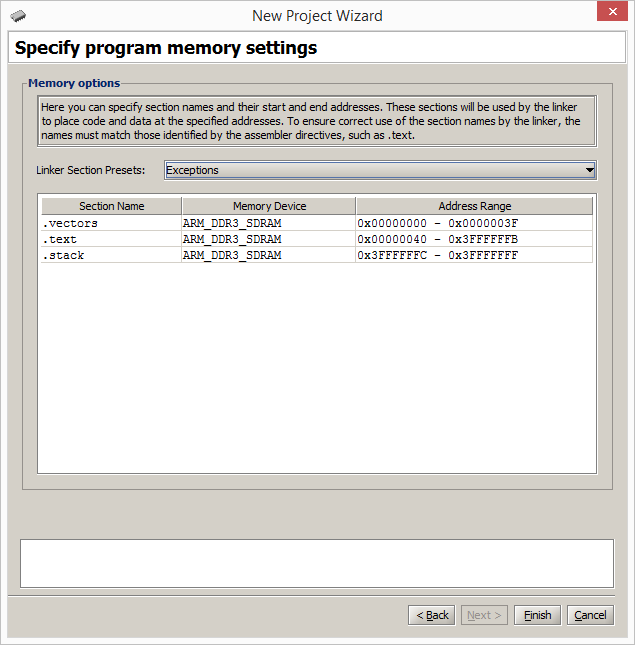
\includegraphics[scale=0.58]{figures/exceptions.png}
	\end{center}
	\vspace{-0.25cm}\caption{Selecting the {\sf Exceptions} linker section.}
\label{fig:exceptions}
\end{figure}

\newpage
\noindent
{\bf Part II}
~\\
~\\
\noindent
Consider the main program shown in Figure~\ref{fig:code2}. The code has to set up 
the ARM stack pointer for interrupt mode, initialize some devices, and then enable interrupts.
The subroutine {\it config\_GIC( )} configures the GIC to send interrupts to the ARM 
processor from two sources: HPS Timer 0, and the pushbutton KEYs port. The main program calls the
subroutines {\it config\_HPS\_timer( )} and {\it config\_KEYS( )} to set up the two ports. You
are to write each of these subroutines. Set up HPS Timer 0 to generate one interrupt
every 0.25 seconds.

~\\
\noindent
In Figure~\ref{fig:code2} the main program executes an endless loop writing the value of
the global variable {\it count} to the red lights LEDR.  In the interrupt service routine for 
HPS Timer 0 you are to increment the variable {\it count} 
by the value of the {\it run} global variable, 
which should be either 1 or 0.  You are to toggle the value of the {\it run} global variable 
in the interrupt service routine for the pushbutton KEYs, each time a KEY is pressed.
When {\it run} = 0, the main program will display a static count on the red lights,
and when {\it run} = 1, the count shown on the red lights will increment every 0.25 seconds.

~\\
\noindent
Make a new folder and Monitor Program project for this part, and assemble, download, and 
test your code.

\begin{figure}[H]
\begin{center}
\lstinputlisting[language=C]{../design_files/part2.c}
\end{center}
\caption{Main program for Part II.}
\label{fig:code2}
\end{figure}

\newpage
\noindent
{\bf Part III}
~\\
~\\
\noindent
Modify your program from Part II so that you can vary the speed at which the counter
displayed on the red lights is incremented. All of your changes for this part should be made
in the interrupt service routine for the pushbutton KEYs. The main program and the rest of
your code should not be changed.

~\\
\noindent
Implement the following behavior. When {\it KEY}$_0$ is pressed, the value of the {\it run}
variable should be toggled, as in Part I. Hence, pressing {\it KEY}$_0$ stops/runs
the incrementing of the {\it count} variable. When {\it KEY}$_1$ is pressed, the rate at which
the {\it count} variable is incremented should be doubled, and when {\it KEY}$_2$ is pressed the
rate should be halved. You should implement this feature by stopping HPS Timer 0 within
the pushbutton KEYs interrupt service routine, modifying the load value used in the
timer, and then restarting the timer.

~\\
\noindent
{\bf Part IV}
~\\
~\\
\noindent
For this part you are to add a third source of interrupts to your program, using the A9
Private Timer. Set up the timer to provide an interrupt every 1/100 of a second. Use this
timer to increment a global variable called {\it time}. You should use the {\it time} variable as
a real-time clock that is shown on the seven-segment displays {\it HEX}$5-0$. Use the format 
\red{MM}:\red{SS}:\red{DD}, where \red{{\it MM}} are minutes, \red{\it SS} are seconds 
and \red{\it DD} are hundredths of a second.
You should be able to stop/run the clock by pressing pushbutton {\it KEY}$_3$.
When the clock reaches \red{59}:\red{59}:\red{99}, it should wrap around to 
\red{00}:\red{00}:\red{00}.

~\\
\noindent
Make a new folder to hold your solution for this part. Modify the main
program from Part~III to call a new subroutine, named {\it config\_priv\_timer( )}, which 
sets up the
A9 Private Timer to generate the required interrupts. To show the {\it time} variable in
the real-time clock format \red{MM}:\red{SS}:\red{DD}, you can use the same approach that was
followed for Part 4 of Lab Exercise 6. In that previous exercise you used polled I/O with
the private timer, whereas now you are using interrupts. One possible way to structure
your code is illustrated in Figure~\ref{fig:code3}. In this version of the code, the 
endless loop in the main program writes the values of variables named {\it HEX\_}3\_0
and {\it HEX\_}5\_4 to the 7-segment displays. 

~\\
\noindent
Using the scheme in Figure~\ref{fig:code3}, the interrupt service routine for the private 
timer has to increment the {\it time} global variable, and also update  
the {\it HEX\_}3\_0 and {\it HEX\_}5\_4 variables that are being written to the 
7-segment displays by the main program.

~\\
\noindent
Make a new Monitor Program project and test your code. 

\begin{figure}[H]
\begin{center}
\lstinputlisting[language=C]{../design_files/part4.c}
\end{center}
\vspace{-0.5cm}\caption{Main program for Part IV.}
\label{fig:code3}
\end{figure}



%%%%%%%%%%%%%%%%%%%%%%%%%%%%%%%%%%%%%%%%
%%% FPGAcademy Copyright Information %%%
%%%%%%%%%%%%%%%%%%%%%%%%%%%%%%%%%%%%%%%%

%Always put the copyright on a new page (clear page), with some vertical space from top
\clearpage
\vspace{1in}

\noindent

Copyright {\copyright} FPGAcademy.org. All rights reserved. FPGAcademy and the 
FPGAcademy logo are trademarks of FPGAcademy.org.  This document is provided 
"as is", without warranty of any kind, express or implied, including but not 
limited to the warranties of merchantability, fitness for a particular purpose 
and noninfringement. In no event shall the authors or copyright holders be 
liable for any claim, damages or other liability, whether in an action of 
contract, tort or otherwise, arising from, out of or in connection with the 
document or the use or other dealings in the document.
~\\
~\\
**Other names and brands may be claimed as the property of others.


\end{document}
